\documentclass[12pt]{article}
\usepackage[spanish]{babel}
\usepackage{apacite}
\usepackage[utf8]{inputenc}
\usepackage{amsmath}
\usepackage{amsfonts} 
\usepackage{newtxtext,newtxmath}
\usepackage{listings}
\usepackage[usenames]{color}
\definecolor{gray97}{gray}{.97}
\definecolor{gray75}{gray}{.75}
\definecolor{gray45}{gray}{.45}
\definecolor{azul1}{RGB}{141,198,163}
\definecolor{azul2}{RGB}{24,107,122}
\definecolor{verde1}{RGB}{44,186,34}
\usepackage{textcomp}
\lstset{
		frame=Ltb,
		framerule=1pt,
		framextopmargin=5pt, %margen de arriba
		framexbottommargin=5pt, %margen de abajo
		framexleftmargin= -2pt, %separacion del margen izquierdo
		framesep=2pt,
		rulesep=0.2pt,
		backgroundcolor=\color{gray97},
		rulesepcolor=,
        tabsize=4,
        rulecolor=\color[RGB]{106, 182, 217}, %AZUL
        upquote=true,
        aboveskip={1.5\baselineskip}, %despues de la linea de texto
        columns=fixed,
        showstringspaces=false,
        extendedchars=true,
        breaklines=true,
        prebreak = \raisebox{0ex}[0ex][0ex]{\ensuremath{\hookleftarrow}},
        showtabs=false,
        showspaces=false,
        showstringspaces=false,
        basicstyle=\scriptsize\ttfamily\color[RGB]{39, 100, 46}, %Numeros de lineas, simbolos, puntos y coma y demas
        identifierstyle=\ttfamily\color[RGB]{56, 140, 189}, %variables
        commentstyle=\color[RGB]{62, 179, 101}, %comentarios
        stringstyle=\color[RGB]{247, 165, 42}, %impresiones
        keywordstyle=\bfseries\color[RGB]{237, 118, 150}, %funciones
        %
		numbers=left,
		numbersep=-7pt, %separacion del numero
		numberstyle=\tiny,
		numberfirstline = false,
		breaklines=true,
		}
\usepackage{graphicx}
\usepackage[colorinlistoftodos]{todonotes}
\usepackage{natbib} %citas bibliograficas estilo APA :p
\usepackage{eso-pic}
\usepackage{avant}
\usepackage[top=2cm,bottom=2cm,left=2.5cm,right=3cm,headsep=8pt,a4paper]{geometry}
\usepackage{fancyhdr}
\pagestyle{fancy}
\fancyhf{}
%\fancyhead[LE,RO]{}
\fancyhead[RE,LO]{Robótica}
\fancyfoot[CE,CO]{\leftmark}
\fancyfoot[LE,RO]{\thepage}
\renewcommand{\headrulewidth}{2pt}
\renewcommand{\footrulewidth}{1pt}
\usepackage{tabu}
\usepackage{array}
\usepackage{multirow}
\usepackage{amssymb}
\usepackage{makeidx}
\graphicspath{ {images/} }
\usepackage{wrapfig}
\usepackage{enumerate}
\usepackage{amsmath,tikz}
\usetikzlibrary{matrix}
\usepackage{steinmetz}
\newcommand*{\horzbar}{\rule[0.05ex]{2.5ex}{0.5pt}}
\usepackage{calc}
\date{\today}


\begin{document}

\begin{titlepage}
\newcommand{\HRule}{\rule{\linewidth}{0.5mm}} 
\center
\textsc{\LARGE  Benemérita Universidad \\[0.2cm] Autónoma de Puebla}\\[1.5cm] 

\includegraphics[width=4cm]{IMAGENES/escudo}\\[1cm]
\textsc{\Large Facultad de Ciencias de la Electrónica}\\[0.5cm] 
\textsc{\large Licenciatura en Electrónica}\\[0.5cm]
\HRule \\[0.4cm]
{ \huge \bfseries Cinemática}\\[0.4cm] 
\HRule \\[1.5cm]
\begin{minipage}{\textwidth}
\center 
\textsc{\LARGE Robótica}\\[1.7cm] 
\emph{Profesor:} \\
Dr. Fernando Reyes Cortés \\[1cm]
\begin{tabular}{ll}
\emph{Alumno:} & \emph{Número de Matrícula:}\\
Hanan Ronaldo Quispe Condori  & 555010653\\
\end{tabular}
\end{minipage}\\[2cm]
\today
\end{titlepage}

\newpage
\section{Resumen}
En el presente trabajo se muestra el uso del modelo cinemático directo de un robot prototipo, para comenzar se calculo su tabla de Denavit–Hartenberg, con estos parametros se uso la forma general de la matriz de transformación homogénea esto con la ayuda de una transformación auxiliar como se hizo en el caso del robot cartesiano desarrollado en clase debido a la dificultad que presenta la posición de casa planteada, el determinante del jacobiano nos indicó los puntos singulares dada la posición de casa propuesta y con ayuda de la cinemática inversa y las ecuaciones paramétricas de la elipse se logro el grafico de esta cónica en el plano $xy$ .
\newpage
\section{Propositos}
\begin{itemize}
    \item Generales.
    \begin{itemize}
        \item Hacer uso del modelo cinemático del robot prototipo planteado para realizar el recorrido de una elipse en un plano a elección. 
    \end{itemize}
    \item Particulares
    \begin{itemize}
        \item Calcular la tabla de Denavit–Hartenberg.
        \item Calcular la matriz homogénea del robot prototipo planteado.
        \item Calcular el jacobiano del robot prototipo planteado.
        \item Calcular las ecuaciones de cinemática inversa del robot prototipo planteado.
    \end{itemize}
\end{itemize}
\newpage
\section{Introducción}
La cinemática es la parte de la física que estudia el movimiento de los cuerpos, sin tomar en cuenta las fuerzas que lo originan, esto nos indica que no se tomarán en cuenta ecuaciones diferenciales como era el caso de los modelos dinámicos.
\vspace{6mm}

Los robots industriales estan compuestos por una serie consecutiva de eslabones y articulaciones para formar una cadena en cinemática abierta, la cual es la estructura mecánica básica de un robot industrial. La cadena cinemática abierta esta conformada por los siguientes elementos: La primera articulación sirve para formar la base, luego siguen las conexiones sucesivas entre articulaciones y eslabones, finalmente el extremo del último eslabon no posee una articulación, por lo general aqui se coloca la herramienta de trabajo segun lo requiera una aplicacion en específico[\cite{reyes2011robotica}].
\vspace{6mm}

Las articulaciones se constituyen de un servomotor, estos representan las interconexiones entre dos eslabones concecutivos. Una articulación puede realizar solo un tipo de movimiento, este puede ser lineal, tambien llamada prismática, o rotacional [\cite{reyes2011robotica}].
\vspace{6mm}

Al estudio de la cinemática aplicado a los sistemas mecánicos que forman robots manipuladores se le denomina cinemática directa, esta se refiere al estudio analítico del movimiento del robot con respecto a un sistema de referencia cartesiano fijo, [\cite{reyes2011robotica}].
\vspace{6mm}

De manera general, el posicionamiento del extremo final del robot en el espacio tridimensional requiere de seis coordenadas, de estas tres se utilizan para la posición cartesiana y las otras tres se utilizan para la orientación de la herramienta de trabajo.
\\
Dependiendo de la aplicacion del robot se pueden requerir menos coordenadas, ya que algunas de ellas podrian tener el valor de cero y por lo tanto no seria necesario incluirlas en el calculo matemático.
\vspace{6mm}

La cinemática inversa representa en la robótica un area de mayor complejidad que la cinemática directa.
\\
Para un robot manipulador siempre es posible encontrar el modelo de cinemática directa mientras que en la cinemática inversa puede haber varias soluciones o no existir solución analítica, en caso se presente esta situación, serán necesarias otros metodos tales como:
\begin{itemize}
    \item Metodos Numéricos
    \item Redes Neuronales 
    \item Metodos Iterativos 
    \item Metodos Geométricos
\end{itemize}

\textbf{Convención Denavit–Hartenberg}
\vspace{6mm}

Esta es una herramienta usada ampliamente conocida en el area de la robótica y de la ingeniería, esto por que ofrece un procedimiento simple para obtener el modelo cinemático directo, cuya estructura queda en terminos de matrices de transformaciones homogeneas cuyos elementos dependen de los cuatro parametros de Denavit–Hartenberg, en adición a estos parametros se agrego un termino extra $\beta$ que representa al espesor del servomotor [\cite{reyes2011robotica}].

\section{Planteamiento y Descripción del Problema}

\begin{enumerate}
    \item Obtener la tabla DH, considerando la posición de casa indicada en la figura 1, describa la matriz de la transformación homogénea $H_0^3$.
    \begin{figure}[h]
        \centering
        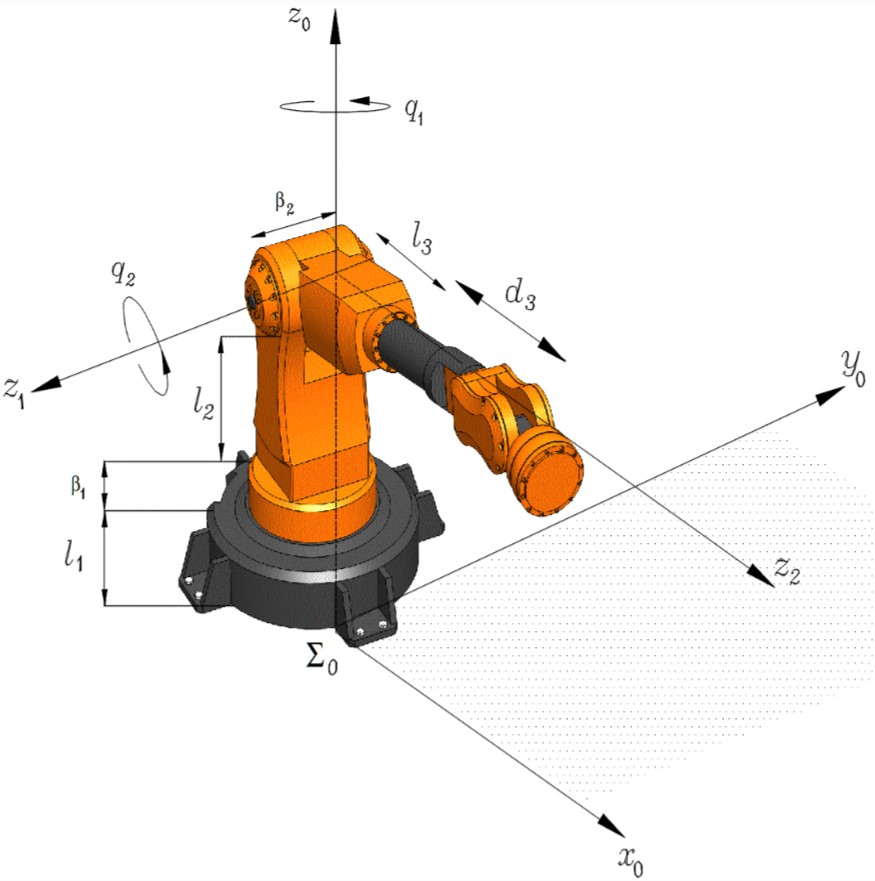
\includegraphics[width=8cm, height=7cm]{IMAGENES/1.jpg}
        \caption{Robot Prototipo.}
        \label{fig:proto}
    \end{figure}
    \item Indique la región dentro del espacio de trabajo donde se encuentran los puntos singulares del robot.
    \item Diseñar una trayectoria elíptica, tal que el extremo final del robot pueda trazar en su espacio de trabajo. Determine los parametros geométricos de la trayectoria (centros, foco, radio, etc) de acuerdo a las dimensiones del robot.
\end{enumerate}
\section{Solución del Problema}
\begin{enumerate}
    \item Se tendran que asignar los sistemas de referencia en la figura \ref{fig:proto}, esto resultará en la siguiente figura.
    \begin{figure}[h]
        \centering
        \includegraphics[width=8cm, height=7cm]{IMAGENES/sist_referencia.eps}
        \caption{Sistemas de Referencia Asignados.}
        \label{fig:reference}
    \end{figure}

    Para realizar esta asignación se tuvo que hacer uso de un sistema de referencia auxiliar, esto ya que la posición de casa propuesta presenta el caso en el que al rotar el eje $z_1$ alrrededor de $x_1$ es imposible llegar $z_2$, cabe mencionar que este es el mismo caso que se presento en el analisis del robot cartesiano desarrollado en clase. 
    \\
    Esta asignación realizo de la siguiente manera.

    \begin{figure}[h]
        \centering
        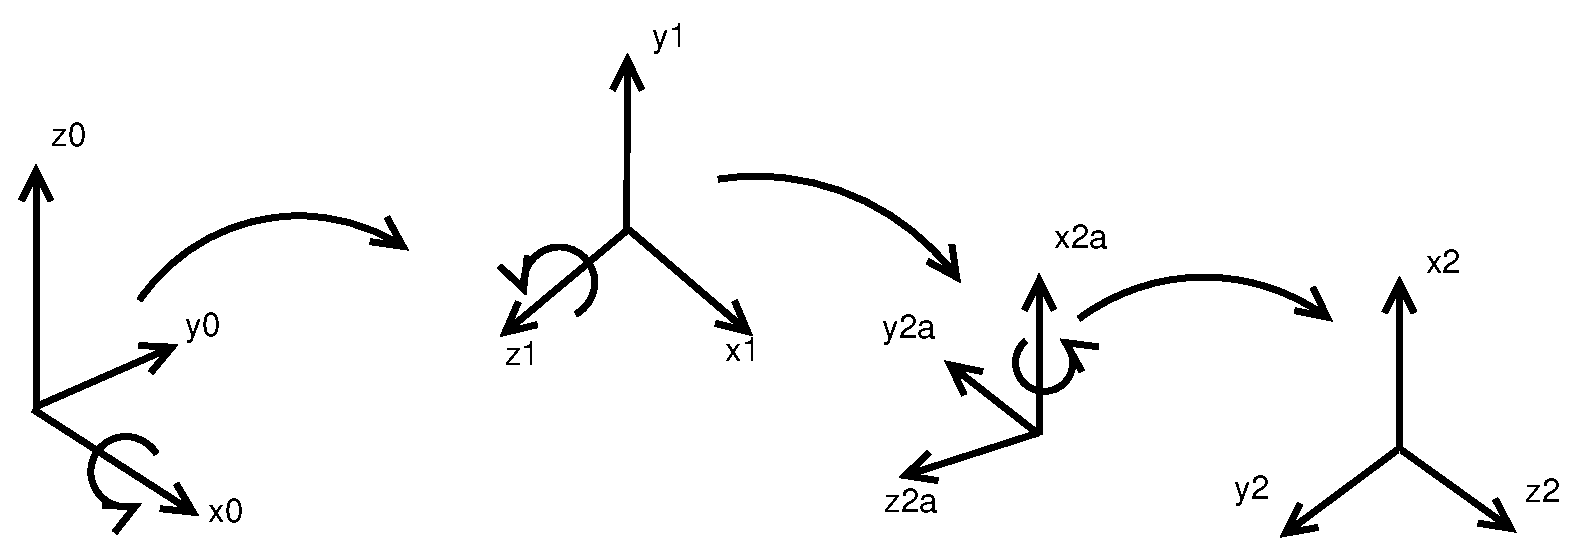
\includegraphics[width=15cm, height=5cm]{IMAGENES/rotacion.eps}
        \caption{Rotación Sistemas de Referencia.}
        \label{fig:rotaciones}
    \end{figure}

    La tabla de Denavit–Hartenberg para el robot de figura \ref{fig:reference} estará dada por

    \begin{center}
        \begin{tabular}{ |c|c|c|c|c| } 
            \hline
            $l$ & $\alpha$ & d,$\beta$ & $\theta$\\
            \hline
            $0$ & $\frac{\pi}{2}$ & $l_1+\beta_1+l_2$ & $q_1$\\ 
            $0$ & $\frac{\pi}{2}$ & $\beta_2$ & $q_2$ \\ 
            $0$ & $0$ & $l_3+d_3$ &$0$ \\ 
            \hline
        \end{tabular}
    \end{center}
    Apartir de estos parametros se pueden hallar las siguientes matrices de transformación homogénea
    \begin{equation}
        \begin{split}
            H_0^1&=
            \begin{bmatrix}
                cos(q_1)&0 & sen(q_1)& 0\\
                sen(q_1)&0&-cos(q_1)&0\\
                0&1&0&l_1+\beta_1+l_2\\
                0&0&0&1
            \end{bmatrix}\\
            H_1^2&=
            \begin{bmatrix}
                cos(q_2)&0 & sen(q_2)& 0\\
                sen(q_2)&0&-cos(q_2)&0\\
                0&1&0&\beta_2\\
                0&0&0&1
            \end{bmatrix}\\
            H_{2a}&=H_{Rz1,\frac{\pi}{2}}*H_1^2\\
            H_{2a}&=
            \begin{bmatrix}
                0&-1&0&0\\
                1&0&0&0\\
                0&0&1&0\\
                0&0&0&1
            \end{bmatrix}*
            \begin{bmatrix}
                cos(q_2)&0 & sen(q_2)& 0\\
                sen(q_2)&0&-cos(q_2)&0\\
                0&1&0&\beta_2\\
                0&0&0&1
            \end{bmatrix}\\
            H_{2a}&=
            \begin{bmatrix}
                -sen(q_2)&0&cos(q_2)& 0\\
                cos(q_2)&0&sen(q_2)&0\\
                0&1&0&\beta_2\\
                0&0&0&1
            \end{bmatrix}\\
            H_2^3&=
            \begin{bmatrix}
                1&0&0&0\\
                0&1&0&0\\
                0&0&1&l_3+d_3\\
                0&0&0&1
            \end{bmatrix}\\
        \end{split}
        \label{eq:trans_homo}
    \end{equation}
    Haciendo uso de las ecuaciones \ref{eq:trans_homo} en $H_0^3=H_0^1*H_{2a}*H_2^3$ se tendrá
    \begin{equation}
        \begin{split}
            H_0^3&=
            \begin{bmatrix}
                cos(q_1)&0 & sen(q_1)& 0\\
                sen(q_1)&0&-cos(q_1)&0\\
                0&1&0&l_1+\beta_1+l_2\\
                0&0&0&1
            \end{bmatrix}*
            \begin{bmatrix}
                -sen(q_2)&0&cos(q_2)& 0\\
                cos(q_2)&0&sen(q_2)&0\\
                0&1&0&\beta_2\\
                0&0&0&1
            \end{bmatrix}*
            \begin{bmatrix}
                1&0&0&0\\
                0&1&0&0\\
                0&0&1&l_3+d_3\\
                0&0&0&1
            \end{bmatrix}\\
            H_0^3&=
            \begin{bmatrix}
                -sen(q_2)cos(q_1)&sen(q_1)&cos(q_1)cos(q_2)&cos(q_1)cos(q_2)*(l_3+d_3)+\beta_2sen(q_1)\\
                -sen(q_2)sen(q_1)&-cos(q_1)&sen(q_1)cos(q_2)&sen(q_1)cos(q_2)*(l_3+d_3)-\beta_2cos(q_1)\\
                cos(q_2)&0&sen(q_2)&sen(q_2)(l_3+d_3)+l_1+l_2+\beta_1\\
                0&0&0&1
            \end{bmatrix}\\
        \end{split}
        \label{eq:homo_matrix}
    \end{equation}
    De esta ultima matriz de pueden separar la matriz de rotación y el vector de traslación 
    \begin{equation}
        \begin{split}
            R_0^3&=
            \begin{bmatrix}
                -sen(q_2)cos(q_1)&sen(q_1)&cos(q_1)cos(q_2)\\
                -sen(q_2)sen(q_1)&-cos(q_1)&sen(q_1)cos(q_2)\\
                cos(q_2)&0&sen(q_2)
            \end{bmatrix}\\
            d_0^3&=
            \begin{bmatrix}
                x\\
                y\\
                z
            \end{bmatrix}=
            \begin{bmatrix}
                cos(q_1)cos(q_2)*(l_3+d_3)+\beta_2sen(q_1)\\
                sen(q_1)cos(q_2)*(l_3+d_3)-\beta_2cos(q_1)\\
                sen(q_2)(l_3+d_3)+l_1+l_2+\beta_1
            \end{bmatrix}\\
        \end{split}
        \label{eq:cine_direc}
    \end{equation}
    El vector de traslación nos dara información sobre la cinematica directa del robot.
    \item Los puntos singulares se calcularán mediante la determinante del jacobiano del vector de traslación, esta se calculará usando $J(q_1,q_2,d_3)$.
    \begin{equation}
        \begin{split}
            \begin{bmatrix}
                x\\
                y\\
                z
            \end{bmatrix}&=
            \begin{bmatrix}
                cos(q_1)cos(q_2)*(l_3+d_3)+\beta_2sen(q_1)\\
                sen(q_1)cos(q_2)*(l_3+d_3)-\beta_2cos(q_1)\\
                sen(q_2)(l_3+d_3)+l_1+l_2+\beta_1
            \end{bmatrix}\\
        \end{split}
        \label{eq:jacobian}
    \end{equation}
    Los elementos de esta matriz estaran dados por 
    \begin{equation}
        \begin{split}
            J_{1,1}&=-sen(q_1)cos(q_2)*(d_3+l_3)+\beta_2cos(q_1)\\
            J_{2,1}&=cos(q_1)cos(q_2)*(d_3+l_3)+\beta_2sen(q_1)\\
            J_{3,1}&=0\\
            J_{1,2}&=-cos(q_1)sen(q_2)*(d_3+l_3)\\
            J_{2,2}&=-sen(q_1)sen(q_2)*(d_3+l_3)\\
            J_{3,2}&=cos(q_2)*(d_3+l_3)\\
            J_{1,3}&=cos(q_1)cos(q_2)\\
            J_{2,3}&=sen(q_1)sen(q_2)\\
            J_{3,3}&=sen(q_2)
        \end{split}
        \label{eq:jacob}
    \end{equation}
    Usaremos Matlab para calcular la determinante de este jacobiano.
    \lstinputlisting[language=Matlab]{Matlab/jacobi.m}
    La salida de este script es la siguiente
    \lstinputlisting[language=Matlab]{Matlab/diary}
    
    De la linea $19$ del resultado tendremos que los puntos singulares estaran dados donde $cos(q_2)*)(d_3+l3)=0$ esto corresponde a los puntos donde $q_2=\pm(2n+1)\pi$ donde $n\in \mathbb{N}$, no existe condicion para $d_3$ ya que al ser una longitud esta nunca puede ser negativa, por lo tanto el segundo factor no puede ser $0$.
    \item Se usaran las ecuaciones parametricas de la elipse en conjunto con la cinemática inversa del robot.
    \begin{equation}
        \begin{split}
            x=a+bcos(t)&\\
            y=c+dsen(t)
        \end{split}
        \label{eq:para_elip}
    \end{equation}
    En la ecuación \ref{eq:para_elip} el centro de la figura estará dado por el par ordenado $a,c$ y tendrá semiejes $b$ y $d$ siendo estos distintos $b\not =d$.  
\end{enumerate}
\section{Conclusiones}
\begin{itemize}
    \item Se puede concluir que las matrices de transformación homogeneas calculadas mediante la convención de Denavit–Hartenberg predicen el comportamiento de la cinemática del robot.
\end{itemize}
\bibliographystyle{apacite}
\bibliography{biblio}
\section{Anexos}
\lstinputlisting[language=Matlab]{Matlab/jacobi.m}
\end{document}